% #############################################################################
%															Bahnplanung und Steuerung
% #############################################################################
\chapter{Bahnplanung und Steuerung}
\label{bahnplanung_steuerung_cha}

% ********************************************************************************
% 										Aufgabenstellung
% ********************************************************************************
\section{Aufgabenstellung}
\label{bahnplanung_aufgabenstellung_sec}
\authorsection{\editoroier}


Was die Aufgabestellung für die Bahnplanung und Steuerung betrifft, so kann man das in Abstraktionsschichten einteilen:
LowLevel-Ansteuerung, Inverse Kinematik, Bahnplanung und Kollisionsvermeidung.
Außerdem sollte man das alles auch Simulieren können.

Für die LowLevel Ansteuerung ist die plattformspezifische Ansteuerung und Simulation notwendig. Außerdem sollte man auch die Pose aus Odometriedaten bestimmen können.

Die inverse Kinematik dient dazu um aus einer gegebene Pose, eine oder mehrere, bis hin zu unendlich vielen Roboterkonfigurationen zu berechnen. Letzteres passiert bei wenn es Raumpunkte gibt die zu Singularitäten führen. Das heißt,  dass zum Beispiel bei einem 6 Achsigen Roboter, zwei Achsen kollinear werden. Im Falle einer mobilen Plattform, würde man als inverse Kinematik die Berechnung einer Radstellung zu einer Pose (x, y, yaw) betrachten. Die Bestimmung der Geschwindigkeit wird danach durch inverse Odometrie gemacht. Zu lösende Aufgaben in Bereich der inverse Kinematik waren: die Umrechnung der Trajektorie in Geschwindigkeiten, die Limitierung der Beschleunigung des Roboters und das Limitieren der Geschwindigkeiten unter Beachtung des Protective Field \ref{sec:vpf}.

Was die Bahnplanung betrifft, gibt es mehrere Aufgaben. Als erstes müssen die Menschendaten, sprich, die Daten von der Kinect Kamera verarbeitet werden. Danach soll die Trajektorie auf der der Roboter fahren soll bestimmt werden, welches nebenbei kollisionsfrei sein sollte. Als letztes sollte das speichern der abgefahrenen Trajektorie und das Laden der abgefahrene Trajektorie implementiert werden.


%Als Ausgangssituation hatte man die Grundlagen der Odete für die LowLevel-Ansteurung und die inverse Kinematik. Sonst waren, Bahnplanung/Steuerung und Kollisionsvermeidung zunächst nicht vorhanden. Eine Simulationsumgebung war vorhanden, es fehlte aber noch die Programmierung der Gui .
%
%Nach dem Bottom-Up Prinzip hat man zunächst, die LowLevel-Ansteuerung von der Odete angepasst und mittels Simulation getestet.

%Das \textit{DriveAlongPath} Modul, welches sich mit der inverse Kinematik beschäftigt, dient um aus eine Trajektorie aus 3 Punkte die nötige Koordinaten für \textit{OmniDrive} zu berechnen.
%Falls es sich bspw. um ein Industrieroboter handeln würde, dann würde die inverse Kinematik die nötige Gelenkwinkeleinstellungen berechnen, um mit dem Greifer eine neue Position zu erreichen.
%Danach würde die inverse Dynamik die entsprechende Motor-Kräfte und Momente berechnen.
%
%Die Bahnplanung berechnet Trajektoriepunkte auf Basis der Mensch-Position und Geschwindigkeit, welche von der Kinect-Kamera geliefert werden.
%Außerdem werden hier diverse Transformationen von Welt zu Roboter bzw. Bild-Koordinaten und zurück gemacht.
%Nebenbei, wird der Pfad gespeichert damit der Roboter es später alleine abfahren kann.
%
%Zum Schluß wird eine ständige Überprüfung der geplante Trajektorie gemacht, um Kollisionen zu vermeiden.
%Um Hindernisse zu umfahren, werden der A*-Algorithmus und ein Potentialfeld eingesetzt.
%Letzteres wirkt, dass es \glqq teuer\grqq \space ist in der nähe von Hindernisse zu fahren.



% ********************************************************************************
% 										Grundlagen Bahnplanung
% ********************************************************************************
\section{Grundlagen der Bahnplanung und Steuerung}


\subsection{Steuerung}
\label{bahnplanung_steuerung_sec}

Weil die gefundene Trajektorie normalerweise nicht glatt ist werden für die Steuerung unterschiedliche Interpolationsarten verwendet. Die Bahnsteuerung kann in Kartesischen Raum oder im Konfigurationsraum stattfinden. In Kartesischen Raum ist es näher an der zu lösenden Aufgabe, man muss dann aber für jeden Punkt die inverse Kinematik berechnen. Die Steuerung in Konfigurationsraum hingegen liegt näher an den Gelenken, dafür ist die Formulierung der Trajektorie umständlicher. Vor und Nachteile beider Optionen kann man auf der Tabelle \ref{fig:steurungProContra} sehen.


\begin{table}[h]
		\centering
		\begin{tabular}{| p{7cm} | p{7cm}|}
\hline
\textbf{Kartesischer Raum} & \textbf{Konfigurationsraum}\\
\hline
+ Bahn einfacher zu formulieren & + Ansteuerung der Gelenke ist
einfacher\\
+ Interpolation ist einfacher & + Trajektorie ist eindeutig und
berücksichtigt Grenzen\\

- Inverse Kinematik ist für jeden Trajektorienpunkt zu lösen & - Interpolation für mehrere
Gelenke\\
- Geplante Trajektorie nicht immer ausführbar & - Formulierung der Trajektorie umständlicher\\
\hline
		\end{tabular}
		\caption{\label{fig:steurungProContra} Vor und Nachteile der Steuerung im Kartesischen und Konfigurationsraum Quelle: \citep{rob1}}
		\end{table}	
Es gibt unterschiedliche Interpolationsarten:  Zirkular, Linear und Spline-Bahn oder auch approximative Bahnsteuerung.
Bei der Linearinterpolation wird einfach zwischen zwei Teiltrajektorien interpoliert wie man auf der Abbildung \ref{fig:linearinterpolation} sehen kann.
\begin{figure}[h]
	\center
	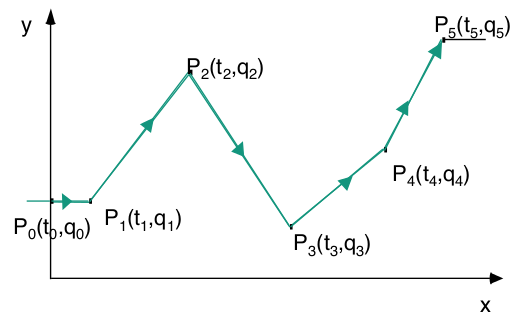
\includegraphics[scale=0.35]{graphics/linearinterpolation.png}
	\caption{\label{fig:linearinterpolation} Beispiel der Linearinterpolation Quelle: \citep{rob1}}
\end{figure}
 Die Zirkularinterpolation schafft hingegen kreisförmige Verfahrwege zwischen zwei Punkte. Wenn man hingegen  Segmentweise interpoliert, werden die Endbedingungen der Teiltrajektorie i-1 und die Anfangsbedingungen der Teiltrajektorie i aneinander angepasst, so dass die Teiltrajektorien durch Splines beschrieben werden wie man auf der Abbildung \ref{fig:segmentinterpolation} sehen kann.
\begin{figure}[h]
	\center
	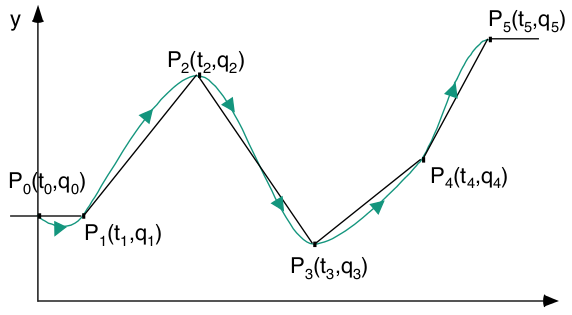
\includegraphics[scale=0.35]{graphics/segmentinterpolation.png}
	\caption{\label{fig:segmentinterpolation} Beispiel der Segmentweise Bahninterpolation Quelle: \citep{rob1}}
\end{figure}
 
 
 Bei der approximative Bahnsteuerung werden anders als bei der Bahninterpolation, nicht alle Kontrollpunkte der Trajektorie befahren, sondern die Kontrollpunkte beeinflussen den Bahnverlauf und werden approximiert. Neben Bernsteinpolynome werden hier besonders Überschleifen benutzt um sanft Kurven zu fahren wie man auf der Abbildung \ref{fig:ueberschleifeninterpolation} sieht. Letzteres wurde auch in Praktikum eingesetzt.
 \begin{figure}[h]
\center
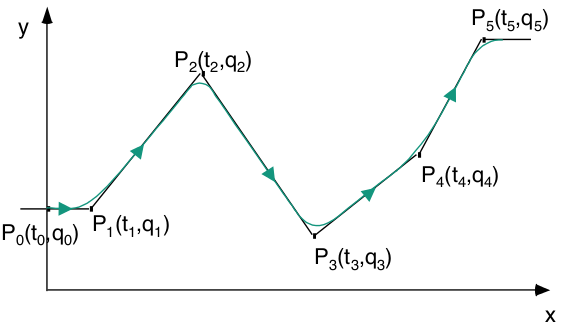
\includegraphics[scale=0.35]{graphics/ueberschleifeninterpolation.png}
\caption{\label{fig:ueberschleifeninterpolation} Beispiel der approximierte Bahnsteuerung mit Überschleifen Quelle: \citep{rob1}}
\end{figure}




\label{bahnplanung_grundlagen_sec}
\authorsection{\editoroier}
\subsection{Bahnplanung}

Bahnplanung befaßt sich mit dem Problem, eine kollisionsfreie Bahn zu finden die  ein Robotersystem
von der aktuellen Position in die Zielposition überführt. Damit gehört es zu einer der Basisprobleme der Robotik. Die Verfahren kann man nach unterschiedliche Gesichtspunkte klassifizieren \cite{rob1}.

Nach Robotertyp:
\begin{itemize}
\item Bahnplanung für Manipulatoren (Schweißen bei Industrierobotern z.B.)
\item Bahnplanung für mobile Roboter
\item Bahnplanung für Laufmaschinen und anthropomorphe Systeme
\item Greif- und Montageplanung
\end{itemize}

Nach dem Zustandsraum wo die Planung stattfindet:
\begin{itemize}
\item Gelenkwinkelzustandsraum (Konfigurationsraum, der Raum alle möglichen Gelenkwinkelkonfigurationen des Roboters )
\item Euklidischer Raum (Arbeitsraum, 3D / 6D)
\item Sensorzustandsraum
\item Objektzustandsraum
\end{itemize}

Nach Vollständigkeit:
\begin{itemize}
\item Vollständige Verfahren (liefern immer eine Korrekte Lösung und können ermitteln ob keine Lösung existiert)
\item Probabilistisch Vollständige Verfahren (Falls eine Lösung existiert konvergiert die Wahrscheinlichkeit, dass eine Lösung gefunden wird, bei fortschreitender Zeit gegen 1. Existiert keine Lösung, kann dies nicht ermittelt werden
)
\end{itemize}

Nach Navigationsart:
\begin{itemize}
\item Globale Pfadplanung bedeutet, eine Trajektorie zum Ziel zu planen wenn dem Roboter eine Karte der Umgebung bevorliegt und er sich dort lokalisieren kann.
\item Lokale Pfadplanung wird eingesetzt um Hindernisse zu umfahren und wird bei mobilen Robotern meist in Konbination mit einem globalen Planer benutzt. 
\end{itemize}

Weil die explizite Berechnung des kollisionsfreien Konfigurationsraum bei Roboter mit mehr Freiheitsgrade als 3 sehr teuer ist, benutzt man oft den impliziten Konfigurationsraum. D. h., dass die Bahnplanung in Konfigurationsraum stattfindet, aber die Kollisionen und Abstände in Arbeitsraum berechnet werden und ins diskretisierte Konfigurationsraum transformiert \citep{innoKonz}. So wird der Konfigurationsraum während der Suche exploriert.

Der Ablauf eines Planungsverfahren ist normalerweise in zwei geteilt\cite{Russell2003}.
\begin{enumerate}
\item Eine Roadmap oder Graph aufbauen mittels \gls{Voronoi}, \gls{Sichtgraphen}, \gls{Zellenzerlegung} oder zufällige Knoten je nach Sampling Strategie(für \gls{PRM} Verfahren\cite{Thrun2005} z.B.).
\item Im Graph ein Weg von Startknoten zum Zielknoten finden mittels A*-Algorithmus oder andere Suchalgorithmen.
\end{enumerate}

\subsubsection{Lokale Planer}
\label{bahnplanung_lokale_planer_sec}


In diesem Abschnitt werden ein Paar gängige lokale Planer vorgestellt.

\paragraph{A*-Algorithmus} 


Der \textit{A*-Algorithmus}\citep{Russell2003} ist eine Erweiterung des \textit{Dijkstra Algorithmus} und gehört zu der Klasse von informierten Graphensuchalgorithmen. Dies heißt, dass es eine Schätzungsfunktion benutzt um die Suche zu lenken. Die Grundidee ist, immer den Knoten zu untersuchen der wahrscheinlich am schnellsten ins Ziel führt. Um den vielversprechendsten Knoten zu ermitteln, werden alle bekannte Knoten mit einer \textit{f(x)} Funktion bewertet und von kleinsten \textit{f}-Wert zum größten sortiert. Der Knoten mit dem kleinsten \textit{f}-Wert wird als nächstes untersucht. 

Um den vielversprechendsten Knoten zu ermitteln wird die Formel
\begin{equation}
 f(x) = g(x) + h(x)
\end{equation}
benutzt. Dabei sind \textit{g(x)} die Pfadkosten von Startknoten bis um \textit{x} zu erreichen und \textit{h(x)} ist die Heuristik, sprich, die Schätzung der Pfadkosten von \textit{x} um den Ziel zu erreichen. Wichtig dabei ist, dass die Heuristik immer optimistisch sein muss, das heißt, dass die Schätzung kleiner oder gleich sein muss als die wirklichen Pfadkosten, weil sonst der Algorithmus nicht mehr optimal ist. Als Heuristik wird oft der Euklidische Abstand oder die Manhattan Distanz benutzt. Auf der Abbildung \ref{fig:a*} kann man eine erfolgreich beendete \textit{A*}-Suche mit angaben zum Ablauf.

\begin{figure}[h]
\center
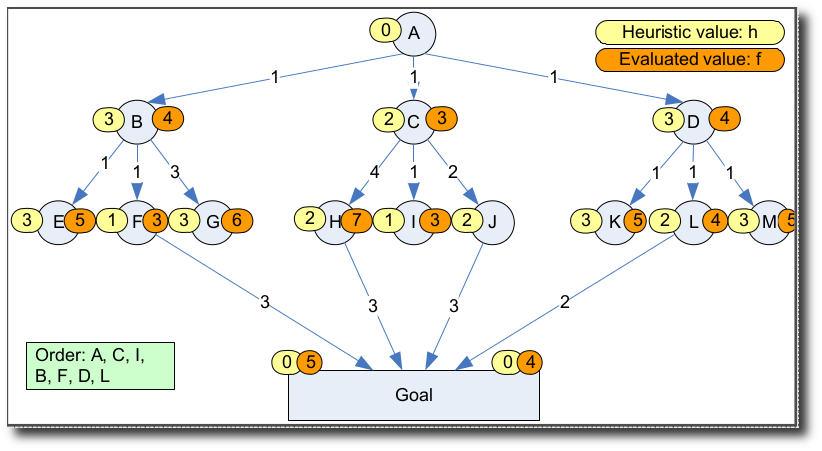
\includegraphics[scale=0.3]{graphics/AStar.png}
\caption{\label{fig:a*} Erfolgreich beendeter Ablauf eines \textit{A*}. Quelle: \citep{innoKonz}}
\end{figure}


Der \textit{A*-Algorithmus}, obwohl es nicht mehr als state-of-the-art gilt\citep{innoKonz},  ist als lokaler Planer, vor allem in 2D, sehr gut. Mit mehr Dimensionen oder Freiheitsgrade performt es viel schlechter. Außerdem kann man den Grundalgorithmus noch sehr viel optimieren. Zum Beispiel mit dem Hierarchischen \textit{A*}, damit es wenn es keine Hindernisse in der nähe liegen größere Schritte und sonst kleinere Schritte macht. Es gibt weitere Erweiterungen für bidirektionale Suche, parallele \textit{A*}-Suche und dynamische Auswahl von Start und Zielknoten. Man könnte auch den Algorithmus stoppen sobald man ein Weg gefunden hat abbrechen, dann ist der Algorithmus natürlich nicht mehr optimal. Diese Erweiterungen sind von den zu lösende Aufgabe abhängig, mehre Start und Zielknoten machen zum Beispiel bei mobilen Robotern nicht viel Sinn, dafür könnte es beim Schweißen nützlich.

\paragraph{Potentialfelder}

Bei diesen Verfahren bewegt sich der Roboter unter dem Einfluss von Kräften, welches ein
Potentialfeld auf ihn ausübt. Die Grundidee ist, dass Hindernisse eine Abstoßungspotential auf den Roboter ausüben und der Ziel hingegen einen Anziehungspotential. Der negative Gradient der resultierende Potentialkraft bestimmt die künstliche Kraft die auf dem Roboter ausgeübt wird.

\begin{equation}
F(q) = - \nabla U(q)
\end{equation}

wo \textit{U(q)} die Summe von den Abstoßungs- und Anziehungspotential ist. Diese Summe ist auf der Abbildung \ref{fig:potentialfeld} dargestellt.


\begin{figure}[h]
\center
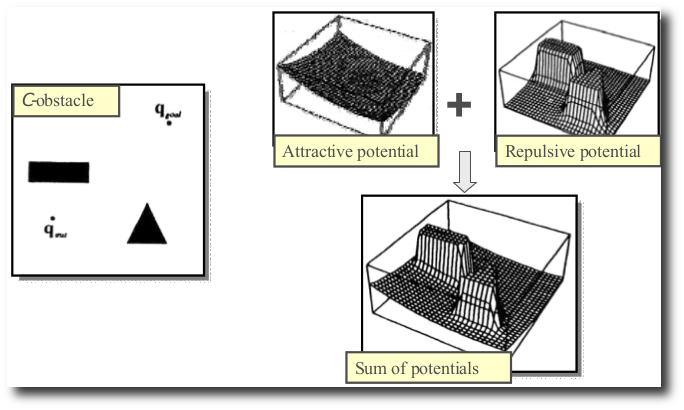
\includegraphics[scale=0.4]{graphics/potentialfeld.png}
\caption{\label{fig:potentialfeld} Summe der Abstoßungs- und Anziehungskräften. Quelle: \citep{innoKonz}}
\end{figure}

Die Vorteile des Verfahren wären zum Beispiel die geringe Rechenaufwand für die Pfadplanung, das die Bahnplanung und Steuerung in einer Funktion verbunden werden\citep{mobileRobotics}, welches die allgemeine Steuerungsstruktur vereinfacht. Noch ein Vorteil ist, dass die Pfade schon glatt sind, sprich, man muss die nicht mehr glätten. Ein Nachteil hingegen ist, das es im lokalen Minima stecken bleiben kann. Dies ist einer der Grunde warum es als lokaler Planer benutzt wird. Um dieses Problem zu beheben muss man Erweiterungen wie  \textit{random walk} oder \textit{backtracking} benutzen. Eine andere Möglichkeit zur Flucht, welches von Rimon und Koditschek vorgestellt wurde, ist den Zielpunkt als einziges lokales Minimum im Potentialfeld zu definieren.




% ********************************************************************************
% 										Umsetzung
% ********************************************************************************
\section{Umsetzung}
\label{bahnplanung_umsetzung_sec}


% -----------------------------------------------------------------------------
%													Motoransteuerung
\subsection{Motoransteuerung}
\label{bahnplanung_motoansteuerung_subsec}
\authorsection{\editoroier}



Was die Motoransteuerung angeht, so gab es schon das plattformunabhängige Modul \lstinline{SegwayOmniHal} von der Odete. Unsere Aufgabe bestand daran, dieses Modul um die plattformspezifische Simulation \lstinline{Segway500RMPSimulation} zu ergänzen. Als Eingang erhält es Geschwindigkeiten und Ausgang sind die Plattformspezifische Geschwindigkeiten. Auf der Abbildung \ref{fig:mca2architecture} sieht man die Gesamte Struktur oder Architektur der Software und auf \ref{fig:segwayHal} ist das Modul \lstinline{SegwayOmniHal} abgebildet.

\begin{figure}[h]
	\center
	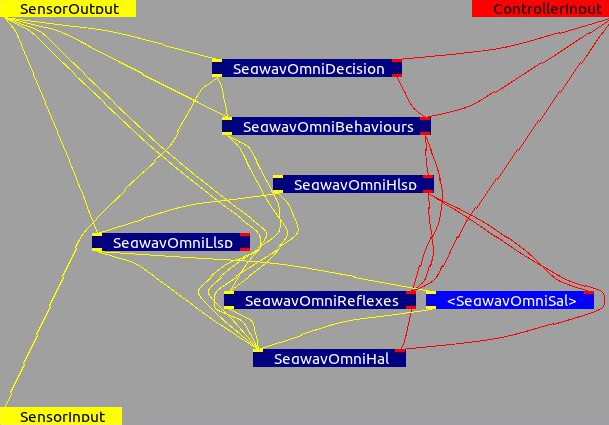
\includegraphics[scale=0.5]{graphics/mca2architecture.png}
	\caption{\label{fig:mca2architecture} Architektur der Software wo man die Vernetzung der einzelnen Module sehen kann}
\end{figure}

\begin{figure}[h]
	\center
	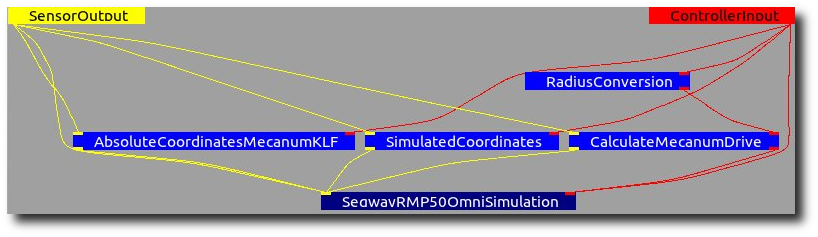
\includegraphics[scale=0.5]{graphics/segwayHal.png}
	\caption{\label{fig:segwayHal} Das Modul \lstinline{SegwayOmniHal}, welches für die Motoransteuerung zuständig ist}
\end{figure}
% evtl. auch so ein Diagramm wie Abb. 4.4 von WS10/11?
%		bzw. Abb. 2.3 von WS09/10


% -----------------------------------------------------------------------------
%													Inverse Kinematik
\subsection{Inverse Kinematik und manuelle Steuerung}
\label{inverse_kinematik_subsec}
\authorsection{\editorjulian}

\todo[inline]{Julian: Schreiben}
In der Gruppe \lstinline{SegwayOmniReflexes} befinden sich die Gruppen für die inverse Kinematik und die manuelle Steuerung des Roboters. Die Ausgaben der beiden Gruppen sind durch einen Multiplexer verbunden, die Selektion erfolgt durch die Berücksichtigung des Status der manuellen Steuerung. Ist diese aktiviert erfolgt unabhängig vom Zustand des Roboters das unmittelbare umschalten auf die manuelle Steuerung und die Ausgabe der Gruppe \lstinline{SegwayOmniManualReflexes} wird verwendet. Ist der manuelle Betrieb nicht aktiv kommt die Ausgabe der Gruppe \lstinline{SegwayOmniAutoReflexes} zur Verwendung. So ist es möglich zu jedem Zeitpunkt den Roboter zu stoppen und ihn manuell zu steuern.

Zur manuellen Steuerung kommt die zur Simulation erstellte \lstinline{MCAGUI} Oberfläche zum Einsatz; beim Test am realen Roboter ein Gamepad.

Die inverse Kinematik bezieht sich auf die \lstinline{MCA2}-Gruppe \lstinline{SegwayOmniAutoReflexes} in der die Umrechnung von einer Trajektorie, bestehend aus drei Koordinaten, in Geschwindigkeiten stattfindet. Die in dieser Gruppe berechneten Geschwindigkeiten sind plattformübergreifend; gehören allerdings einer bestimmten Bewegungsart an. Folgende Bewegungsarten sind möglich:

\begin{description}
	\item[Differentiell] Die Steuerung des Roboters erfolgt indem Antriebsräder auf beiden Seiten des Roboters mit unterschiedlichen Geschwindigkeiten betrieben werden\footnote{\url{http://en.wikipedia.org/wiki/Differential_wheeled_robot}}.
	\item[Omnidirektional] Durch den Einsatz von Mecanum-Rädern\footnote{\url{http://de.wikipedia.org/wiki/Mecanum-Rad}} kann sich der Roboter holonom\footnote{Anzahl der Bewegungsfreiheitsgrade $\geq$ Anzahl Freiheitsgrade, hier: Bewegungsfreiheitsgrade $= 3$, Freiheitsgrade $= 3$.} bewegen.
\end{description}

\begin{figure}[h]
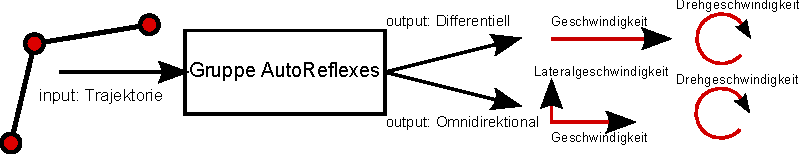
\includegraphics[scale=0.9]{graphics/SCHEMA-invKinem.pdf}
\caption{\label{fig:bahnpl_umsetz_schema_inv_kinem} Schematische Darstellung des in-und Outputs der \lstinline{SegwayOmniAutoReflexes}-Gruppe.}
\end{figure}

Die Ausgabe von dieser Gruppe, also die bewegungsartspezifischen Geschwindigkeiten, werden an die Gruppe für die Motoransteuerung (siehe \ref{bahnplanung_motoansteuerung_subsec}) weitergereicht um plattformspezifische Geschwindigkeiten zu berechnen.

Zusätzlich zur Berechnung der Geschwindigkeiten erfolgt in dieser Gruppe die Begrenzung der tatsächlichen Geschwindigkeit bezüglich einer vorgegebenen maximal Geschwindigkeit sowie der auftretenden Beschleunigungen durch Änderungen der Geschwindigkeit oder Bewegungsrichtung.

Zuletzt findet mit Hilfe des Virtual Protective Field (siehe \ref{lokalisierung_umsetzung_sec}) eine Kollisionsvermeidung statt.

\todo[inline]{Bild der Gruppe mit kurzer Erläuterung bzgl. wo was passiert}

\subsubsection{Vorhandene Software}
\label{bahnplanung_inv_kinem_vorhandene_software_sec}

Im Projekt \lstinline{SegwayOmni} bzw. \lstinline{Odete} gab es bereits eine \lstinline{Reflexes}-Gruppe in der ein Großteil der nötigen Funktionalität implementiert war. Insbesondere der zentrale Teil, die Module \lstinline{DriveAlongPath} bzw. \lstinline{OmniDriveAlongPath} welche für die inverse Kinematik zuständig sind wurden zur Verfügung gestellt. Auch die Module zur Begrenzung der Beschleunigung waren vorhanden und konnten ohne Veränderung integriert werden.

\subsubsection{Erweiterungen}
\label{bahnplanung_inv_kinem_erweiterung_sec}

Um eine einfache Steuerung der Gruppe zu gewährleisten steht an oberster Stelle das Modul \lstinline{AutoReflexesManager}. Dieses Modul vereinfacht und automatisiert verschiedene Funktionen der Module \lstinline{DriveAlongPath}, \lstinline{OmniDriveAlongPath}, \lstinline{Safety} und \lstinline{VirtualProtectiveSafety}:
\todo[inline]{Richtige Namen der modul nachschauen}
\begin{description}
	\item[DriveAlongPath]
	\begin{itemize}
		\item Setzen der maximal Geschwindigkeit
		\item Aktualisieren des Zählers zum Signalisieren das eine neue Trajektorie anliegt
		\item Aktivieren/Deaktivieren des Moduls
	\end{itemize}
	\item[Safety] Aktivieren/Deaktivieren des Moduls
	\item[VirtualProtectiveSafety] Aktivieren/Deaktivieren des Moduls
\end{description}

Weiterhin fließt in der \lstinline{AutoReflexes}-Gruppe die Information aus dem Virtual Protective Field mit ein, um kollisionsfreies Fahren zu ermöglichen.

\subsubsection{Virtual Protective Field}
\label{bahnplanung_virtual_protective_field_sec}

Das Modul \lstinline{VIRTUALPROTECTIVEBLA} ist speziell für den Einsatz beim omnidirektionalen Fahren gedacht. In diesem Fahrmodus berechnet sich der tatsächliche Geschwindigkeitsvektor aus zwei orthogonalen Geschwindigkeitsvektoren, die jeweils die Vorwärtsgeschwindigkeit und die Lateralgeschwindigkeit beschreiben. Das Virtual Protective Field bietet gleichermaßen zu jeder Geschwindigkeitskomponente sowie zur resultierenden Geschwindigkeit die Information ob eine Kollision bevorsteht. Dadurch kann für jede Geschwindigkeitskomponente individuell entschieden werden, ob es nötig ist diese auf null zu setzen, also mit maximaler Bremsbeschleunigung zu bremsen, oder nicht. Durch dieses Vorgehen kann sich der Roboter an Ecken, die durch ungenaue Bahnplanung zu einer Kollision führen würden, vorbei schieben. Zugleich ist es die letzte softwareseitige Barriere, um eine Kollision zu vermeiden.

\todo[inline]{Bild zur Verwendung des Virtual Protective Field}


%\begin{itemize}
%	\item Was konkret passiert -> Umwandlung der Trajektorie in (Plattformunabhängige) Geschwindigkeiten.
%	\item Limitierung der Beschleunigung
%	\item Was geht rein, was kommt raus
%	\item Virtual Protective Field verwenden um kollisionsfrei zu fahren.
%	\item was gab es schon
%	\begin{itemize}
%		\item Modul Reflexes von Odete Projekt
%		\item Bewegungsart abhängige Konvertierung einer Trajektorie
%		\item Differential Drive, Omni Drive
%		\item Safety Modul für Beschleunigung
%	\end{itemize}
%	\item Erweitert um Sicherheitsmodul welches das Virtual Protective Field berücksichtigt
%\end{itemize}


% -----------------------------------------------------------------------------
%													Bahnplanung
\subsection{Bahnplanung}
\label{bahnplanung_subsec}
\authorsection{\editortobias}


% \begin{itemize}
% 	\item Kurzer Grobüberblick über die Behaviours-Gruppe, hier werden Bahnplanungs-Aufgaben bearbeitet\todoprivate{ref zu behaviours-Bild}
% 	\begin{itemize}
% 		\item Berechnung von Trajektorien-Punkten auf Basis der Mensch-Position und Geschwindigkeit (Kinect)
% 		\item Schätzung der zukünftigen Position des Menschen
% 		\item Transformation von Welt- in Roboter- bzw. Bildkoordinaten und zurück\todoprivate{evtl. auch weg lassen}
% 		\item Abspeichern von Pfaden
% 		\item Abfahren von Pfaden
% 	\end{itemize}
% 	\item Module werden im Folgenden kurz beschrieben
% 	\item Kollisionsvermeidung als eigener Abschnitt
% \end{itemize}

Die Aufgaben der Bahnplanung werden in der \lstinline{MCA2}-Gruppe \lstinline{SegwayOmniBehaviours} bearbeitet (s. Abb. \ref{fig:behaviours}).
Im Einzelnen sind dies:
\begin{itemize}
	\item Berechnung von Trajektorien-Punkten auf Basis der Mensch-Position und Geschwindigkeit: \lstinline{GenerateTrajectory}
	\item Schätzung der zukünftigen Position des Menschen: \lstinline{HumanPosition}
	\item Abspeichern von Pfaden: \lstinline{StoreRoboterPositionsToFile}
	\item Abfahren von Pfaden: \lstinline{LoadRoboterPositionsFromFile}
	\item Kollisionsvermeidung: \lstinline{ObstacleAvoidance}
\end{itemize}

\begin{figure}[h]
	\center
	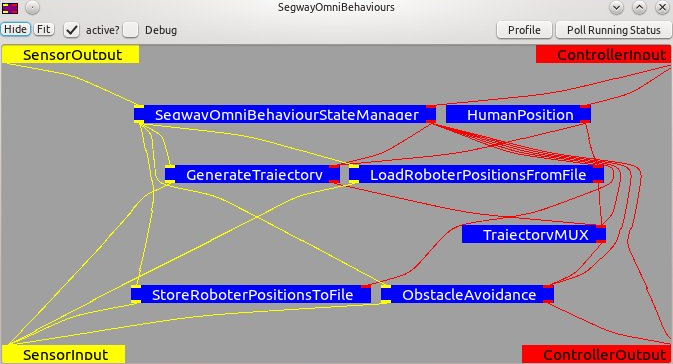
\includegraphics[width=0.8\textwidth]{graphics/behaviours}
	\caption{Die \lstinline{MCA2}-Gruppe \lstinline{SegwayOmniBehaviours}}
	\label{fig:behaviours}
\end{figure}

Die Module innerhalb der Gruppe werden im Folgenden beschrieben.
Die Kollisionsvermeidung wird in einem gesonderten Abschnitt (s. Abs. \ref{kollisionsvermeidung_subsec}) behandelt.


\subsubsection{Position des Menschen}
\label{bahnplanung_humanPosition_subsubsec}

% \begin{itemize}
%     \item bekommt aktuelle Position und Geschwindigkeit des Menschen von Kinect
%     \item schätzt die zukünftige Position des Menschen anhand dieser Daten
%     \item gibt aktuelle und geschätzte Position des Menschen aus
%     \item Zeit-Parameter für die Schätzung: $t_{est}$
%     \item Berechnung nach der Formel: $s_{est} = s_{act} + v \cdot t_{est}$
% \end{itemize}

Das Modul \lstinline{HumanPosition} bekommt als Parameter die aktuelle Position sowie die aktuelle Geschwindigkeit der vom Roboter verfolgten Person übergeben.
Anhand dieser Daten wird die zukünftige Position des Menschen geschätzt.
Als Resultat gibt das Modul die geschätzte zukünftige Position des Menschen aus.
Die aktuelle Position wird ebenfalls mit ausgegeben.

Für die Berechnung der zukünftigen Position des Menschen wird die Formel
\begin{equation}
	s_{est} = s_{act} + v \cdot t_{est}
\end{equation}
angewendet.
$s_{est}$ ist dabei die geschätzte zukünftige Position, $s_{act}$ beschreibt die aktuelle Position und $v$ die Bewegungsgeschwindigkeit des Menschen.
$t_{est}$ ist ein Parameter für die Zeitspanne, die in die Zukunft prädiziert werden soll.
Dieser Parameter wird aus einer externen Konfigurationsdatei geladen.


\subsubsection{Berechnung der Trajektorie}
\label{bahnplanung_trajektorie_subsubsec}

Die Berechnung der Trajektorie erfolgt im Modul \lstinline{GenerateTrajectory}.
Die aktuelle und geschätzte Position des Menschen, sowie die aktuelle Position des Menschen werden als Parameter übergeben, und dienen als Grundlage für die Berechnung der Trajektorie.
Die Struktur der zu berechnenden Trajektorie $s$ ist durch das Modul \lstinline{OmniDriveAlongPath} (s. Abs. \ref{bahnplanung_motoansteuerung_subsec}) vorgegeben:

% \begin{equation}
% 	s =
% 	\begin{pmatrix} start \\ next \\ following \end{pmatrix} =
% 	\begin{pmatrix} x_{st} & y_{st} & 0 \\ x_{nx} & y_{nx} & yaw_{nx} \\ x_{fl} & y_{fl} & 0 \end{pmatrix}
% \end{equation}
% 
% \todo[inline]{welche Variante nehmen?}

\begin{equation}
	s =	\begin{pmatrix} start \\ next \\ following \end{pmatrix}
\end{equation}
mit 
\begin{equation}
	start = 		\begin{pmatrix}	x_{start} \\ y_{start}							\end{pmatrix},
	next = 			\begin{pmatrix} x_{next} \\ y_{next} \\ yaw_{next}	\end{pmatrix},
	following =	\begin{pmatrix}	x_{following} \\ y_{following}							\end{pmatrix}
\end{equation}
Die drei Trajektorien-Punkte sind Ortsangaben mit einer $x$- bzw. $y$-Koordinate.
$following$ beinhaltet zusätzlich eine Komponente für $yaw$ (die ``Blickrichtung'' des Roboters, s. Abb. \ref{fig:roll_pitch_yaw}).

\begin{wrapfigure}{r}{0.35\textwidth}	%\begin{figure}[h]
	\center
	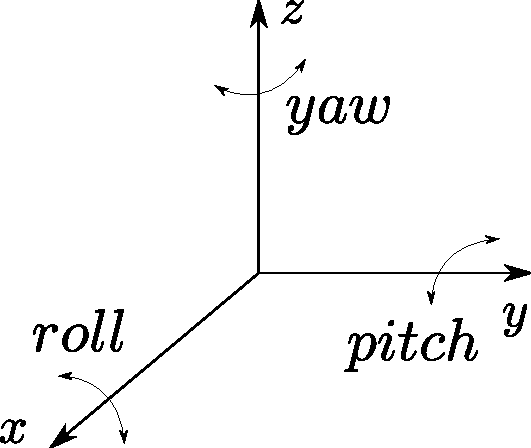
\includegraphics[width=0.3\textwidth]{graphics/roll_pitch_yaw.pdf}
	\caption{Roll-Pitch-Yaw-Winkel \cite{rollPitchYaw}}
	\label{fig:roll_pitch_yaw}
\end{wrapfigure}	%\end{figure}

Die Berechnung einer neuen Trajektorie wird durchgeführt, sobald neue Daten vom Modul \lstinline{HumanPosition} vorliegen.
Als $start$-Punkt wird dabei die aktuelle Roboterposition verwendet.
$next$ ist eine Roboter-Pose, die sich im Abstand $d_{hum}$ vor dem Menschen auf dem Vektor Roboter-Mensch befindet.
Im Abstand $d_{hum}$ vor der geschätzten zukünftigen Mensch-Position auf dem Vektor next-estimated befindet sich der dritte Punkt der Trajektorie: $following$.
Der Abstand $d_{hum}$ zum Menschen kann dabei als externer Parameter vorgegeben werden, der Wert beträgt standardmäßig $1,75m$.
In Abb. \ref{fig:trajektorie} wird dies in einer Schemazeichnung dargestellt.

\begin{figure}[h]
	\center
	% Trajektorien-Punkte der Bahnplanung
% Author : Tobias Roth

\newcommand\Punkt{\tikz[scale=0.07]\draw[thick](-1,-1)--(1,1)(-1,1)--(1,-1);} 

\begin{tikzpicture}


\def \dHum {1.5}

% Definition der Koordinaten für Roboter, Mensch_act und Mensch_est
\def \rX {0}
\def \rY {0}
\def \hActX {3}
\def \hActY {4}
\def \hEstX {8}
\def \hEstY {4}

% Setzen der Koordinaten für Roboter, Mensch_act und Mensch_est
\coordinate (r) at (\rX,\rY);
\coordinate (hact) at (\hActX,\hActY);
\coordinate (hest) at (\hEstX,\hEstY);

% Berechnung der Trajektorien-Punkte
\coordinate (trajPointA) at (r);
\coordinate (trajPointB) at (2.1, 2.8);	% hart codiert..
\coordinate (trajPointC) at (6.53095, 3.70137);	% hart codiert..

% Poitionen zeichnen
\node at (r) (R) {\Punkt};
\node[scale=0.9] at (r) [anchor=east] {$R$};
\node at (hact) (H_act) {\Punkt};
\node[scale=0.9] at (hact) [anchor=south east] {$H_{act}$};
\node at (hest) (H_est) {\Punkt};
\node[scale=0.9] at (hest) [anchor=south west] {$H_{est}$};

\node[scale=0.9] at (r) [anchor=west] {$A$};
\node at (trajPointB) (B) {\Punkt};
\node[scale=0.9] at (trajPointB) [anchor=north] {$B$};
\node at (trajPointC) (C) {\Punkt};
\node[scale=0.9] at (trajPointC) [anchor=north] {$C$};

% Vektoren zwischen Positionen
\path[name path global=rHact, -] (r) edge (hact);
\path[-] (hact) edge (hest);

% d_{Hum} zeichnen
\draw [name path global=hactCircle] (hact) circle (\dHum);
\draw [name path global=hestCircle] (hest) circle (\dHum);
\path[<->] (hact) edge node {$d_{hum}$} (\hActX,\hActY + \dHum);
\path[<->] (hest) edge node {$d_{hum}$} (\hEstX,\hEstY + \dHum);

% Eigentliche Trajektorie zeichnen
\path[red, thick, ->] (trajPointA) edge (trajPointB);
\path[red, thick, ->] (trajPointB) edge (trajPointC);



% Eigentliche Trajektorie zeichnen
% \path [name intersections={of=rHact and hactCircle, by={A}}];
% \node at (A) [below] {$A$};
% \path [name intersections={of=hactCircle and rHact}];
% \coordinate [label=above:$C$] (C) at (intersection-0);


\end{tikzpicture}

	\caption{Berechnung der Trajektorien-Punkte}
	\label{fig:trajektorie}
\end{figure}

Der $yaw$-Wert wird so berechnet, dass der Roboter sich immer in Richtung des Menschen ausrichtet.
So kann gewährleistet werden, dass die Kinect den Menschen weiterhin im Fokus hat.


% \begin{itemize}
% 	\item Modul bekommt aktuelle und geschätzte Position des Menschen, sowie aktuelle Position des Roboters
% 	\item Struktur der zu berechnenden Trajektorie duch \lstinline{OmniDriveAlongPath} \todoprivate{ref zu LowLevel?}\ vorgegeben:
% 	\begin{itemize}
% 		\item Start $(x,y)$, Koordinaten
% 		\item Following $(x,y,yaw)$, Koordinaten und Orientierung \todoprivate{Skizze zu x-y-z-roll-pitch-yaw ?}
% 		\item Next $(x,y)$, Koordinaten
% 	\end{itemize}
% 	\item Berechnung einer neuen Trajektorie, sobald neue Mensch-Daten vorliegen
% 	\item Berechnung der Trajektorien-Punkte im Einzelnen:
% 	\begin{itemize}
% 	  \item Start: aktuelle Roboterposition
% 	  \item Next: Pose auf Roboter-Mensch-Vektor, die sich im Abstand $d$ vor dem Mensch befindet; yaw wird gesondert berechnet, sodass Roboter immer zu Mensch schaut
% 	  \item Following: Position auf next-estimated-Vektor, die sich $d$ vor geschätzter Mensch-Position befindet
% 	  \item erfolgt alles in absoluten Weltkoordinaten
%   \end{itemize}
%   \item Parameter $d$ für den Abstand des Roboters zum Menschen, default: $1,75m$
%   \item Berechnung des yaw-Wertes: \todoprivate{Formel dazu}

% 	\item MUX für Trajektorie
% 	\begin{itemize}
% 		\item GenerateTrajectory
% 		\item LoadFromFile
% 	\end{itemize}
% \end{itemize}


\subsubsection{Pfadspeichern und -laden}
\label{bahnplanung_pfadSpeichernLaden_subsubsec}

% \begin{itemize}
%   \item Im \lstinline{followPerson} -Zustand: Wegpunkte $(x,y,yaw)$ werden in gewissen Abständen $d_{save}$ gespeichert
%   \begin{itemize}
%     \item sobald $ \overline{ s_{act} - s_{last} } > d_{save} $ \todoprivate{Fehler im Code??? Euklidischer Abstand stattdessen verwenden?}
%   \end{itemize}
% 	\item Im \lstinline{loadPath} -Zustand: Nächster Wegpunkt wird geladen, sobald vorheriger erreicht wurde
%   \begin{itemize}
% 		\item Im \lstinline{returnHome} -Zustand: Nächster Wegpunkt wird geladen, sobald vorheriger erreicht wurde; umgekehrte Reihenfolge
%     \item sobald $ d( s_{foll} - s_{act} ) < d( s_{nxt} - s_{act} ) $, Euklidischer Abstand
%   	\item \lstinline{yaw} wird unabhängig von Datei berechnet, sodass Roboter immer Menschen anschaut
%   \end{itemize}
%   \item Eigene Klasse zum File-Handling: \lstinline{fileUtil}
%   \begin{itemize}
%     \item Mehrere dump-files möglich
%     \item Auslesen der Wegpunkte in normaler und umgekehrter Reihenfolge
%   \end{itemize}
% \end{itemize}

Zur Pfadspeicherung bzw. zum Laden eines abgespeicherten Pfades werden zwei Module, sowie eine Helfer-Klasse verwendet:
\begin{itemize}
	\item \lstinline{StoreRoboterPositionsToFile}: Während dem Modus \lstinline{followPerson} (s. Abs. \ref{umsetzung_integration_sec} für weitere Informationen zur globalen Zustandsmaschine) aktiv\todoprivate{evtl. ref noch auf subsec}
	\item \lstinline{LoadRoboterPositionsFromFile}: Während dem Modus Während dem Modus \lstinline{followPath} (s. Abs. \ref{umsetzung_integration_sec}) aktiv\todoprivate{evtl. ref noch auf subsec}
	\item \lstinline{fileUtil}
\end{itemize}

Im globalen Modus \lstinline{followPerson} (s. Abs. \ref{umsetzung_integration_sec}\todoprivate{evtl. ref noch auf subsec}), also während dem Einlernen eines neuen Pfades, schreibt das Modul \lstinline{StoreRoboterPositionsToFile} in regelmäßigen Abständen $d_{save}$ Roboterposen in eine externe Datei (sog. \lstinline{dumpFile}).
Für die Posen werden dabei sowohl die $x$- und $y$-Koordinaten, als auch die $yaw$-Werte abgespeichert.
Der Zeitpunkt für die Abspeicherung der nächsten Pose wird anhand des euklidischen Abstands festgelegt:
Sobald der Abstand der aktuellen Roboterpose zur letzten Speicherpose größer als der Speicherabstand $d_{save}$ ist, wird die aktuelle Pose abgespeichert.
$d_{save}$ kann als Parameter in einer externen Konfigurationsdatei definiert werden.
\begin{equation}
	\| s_{act} - s_{last}\|_2 \quad > \quad d_{save}
\end{equation}

Innerhalb des \lstinline{dumpFile}s werden die $x$, $y$ bzw. $yaw$-Werte durch Doppelpunkte abgetrennt gespeichert.
Eine beispielhafter abgespeicherter Pfad ist in Listing \ref{lst:dump_file} dargestellt.
\todoprivate{Beispiel-Ausschnitt aus dump-file}
\begin{lstlisting}[caption=Beispiel für ein \lstinline{dumpFile} zur Speicherung eines Pfades, label=lst:dump_file]
	1111:2222:3333
	999:888.8:77.77
\end{lstlisting}

Im globalen Modus \lstinline{loadPath} (s. Abs. \ref{umsetzung_integration_sec}\todoprivate{evtl. ref noch auf subsec}), also während dem Abfahren eines gespeicherten Pfades, liest das Modul \lstinline{LoadRoboterPositionsFromFile} die Punkte aus dem \lstinline{dumpFile}.
Der euklidische Abstand findet wieder Verwendung, um den Zeitpunkt festzulegen, an welchem der nächste Punkt in die Trajektorie aufgenommen wird.
Dies geschieht, sobald der Abstand des Roboters zu $following$ kleiner ist als der zu $next$:
\begin{equation}
	\| s_{foll} - s_{act} \|_2 \quad < \quad \| s_{next} - s_{act} \|_2
\end{equation}
Im Modus \lstinline{returnHome} werden die Punkte in umgekehrter Reihenfolge ausgegeben.

In der aktuellen Implementierung werden die aus dem \lstinline{dumpFile} gelesenen $yaw$-Werte \emph{nicht} für die Trajektorie verwendet.
Grund hierfür ist die Entscheidung, dass der Roboter (bzw. die darauf installierte Kinect) immer den Menschen im Fokus behalten soll, um evtl. kurzfristige Stop-Kommandos empfangen und umsetzen zu können.
Die $yaw$-Werte, die während des Pfad-Einlernens abgespeichert wurden, beziehen sich auf die Standpunkte des Menschen zum dortigen Zeitpunkt, und nicht auf die aktuell relevanten Mensch-Positionen. 
Aus diesem Grund werden die $yaw$-Werte innerhalb des \lstinline{LoadRoboterPositionsFromFile}-Moduls auf Basis der aktuellen Mensch-Position gesondert berechnet.

Für die Aufgaben des Datei-Handlings wurde eine eigene Klasse implementiert, die Operationen wie Datei anlegen, öffnen, schließen, in die Datei schreiben, aus der Datei lesen etc. kapselt.
Hier werden die Daten aus der Datei gepuffert, sodass beispielsweise im Fall des Pfad-Lesens nur ein einmaliger Dateizugriff auf Betriebssystem-Ebene erfolgt.
Es ist auch möglich, mehrere \lstinline{dumpFile}s anzulegen.


% 
% % -----------------------------------------------------------------------------
% %													Transformationen
% \subsection{Transformationen}
% \label{transformationen_subsec}
% 
% \authorsection{\editorjulian}
% \todo[inline]{Julian: Sollen wir (also du ;-) ) noch so einen Abschnitt machen?}



% -----------------------------------------------------------------------------
%													Kollisionsvermeidung
\subsection{Kollisionsvermeidung}
\label{kollisionsvermeidung_subsec}

\subsubsection{Modul}
\authorsection{\editortobias}

% \begin{itemize}
%   \item Kollisionsvermeidungsmodul (\lstinline{ObstacleAvoidance}) überprüft die geplante Trajektorie auf Hindernisse, und plant ggf. um Hindernisse
%   \item Ausgaben von \lstinline{GenerateTrajectory} und \lstinline{LoadFromFile} werden geMUXt
%   \begin{itemize}
%     \item je nach Modus (\lstinline{followPerson} bzw. \lstinline{returnHome} / \lstinline{followPath}) schaltet MUX andere Eingänge durch
%   	\item Die Ausgabe des MUX wird dann widerum komplett durch das Kollisionsvermeidungsmodul (\lstinline{ObstacleAvoidance}) geschleift
%     \item Dadurch wird jede Trajektorie auf Hindernisse überprüft, keine kommt \glqq daran vorbei\grqq
%   \end{itemize}
%   \item Innerhalb des Moduls wird jede Trajektorie auf Hindernisse überprüft
% 	\begin{itemize}
% 	  \item die (Bild-)Punkte zwischen start, next und following werden berechnet (Transformation der Welt- in Bildkoordinaten)
% 	  \item Überprüfung für jeden einzelnen Punkt, ob er innerhalb eines Hindernisses liegt
% 	  \item Verwendung der \lstinline{ObstacleMap} \todoprivate{ref zu Lokalisierung}
% 	\end{itemize}
%   \item Ohne Hindernis werden Trajektorien-Punkte nur durchgeschleift
%   \item Wenn Hindernis erkannt, dann wird eine neue Trajektorie ermittelt
%   \begin{itemize}
%     \item Verwendung des A*-Algorithmus
%     \item Ermittlung des Start- und Endpunktes für A*
%     \item ggf. gesonderte Behandlung für Endpunkt (\lstinline{choosePointAfterObstacle})
%     \item Aufruf A*
%     \item Transformation der nuen Trajektorie IK $\rightarrow$ WK
%   \end{itemize}
% \end{itemize}

Das Modul \lstinline{ObstacleAvoidance} überprüft die geplante Trajektorie auf Hindernisse, und plant ggf. um ein Hindernis herum, um Kolissionen zu vermeiden.
Jede von \lstinline{GenerateTrajectory} bzw. \lstinline{LoadRoboterPositionsFromFile} (s. Abs. \ref{bahnplanung_trajektorie_subsubsec}) ausgegebene Trajektorie wird innerhalb des Moduls \lstinline{ObstacleAvoidance} auf Hindernisse überprüft, bevor sie an tiefer liegende Schichten weiter gegeben wird.
Dies wird durch einen \gls{mux} erreicht, der je nach globalem Modus die entsprechenden Eingänge an das Modul \lstinline{ObstacleAvoidance} durchschaltet.
So wird sichergestellt, dass ungeprüfte Trajektorien nicht an die Motoransteuerung weiter gegeben werden.
In Abb. \ref{fig:behaviours} (S. \pageref{fig:behaviours}) ist das Modul innerhalb der \lstinline{Behaviours}-Gruppe sichtbar.

Für die Hindernis-Überprüfung innerhalb des Moduls werden die Trajektorienpunkte, die alle in \gls{wk} vorliegen, in \gls{bk} transformiert.
So werden $start$, $next$ und $following$ auf entsprechende Punkte der \lstinline{ObstacleMap} (s. Abs. \ref{hinderniskarte_subsec}, S: \pageref{hinderniskarte_subsec}) abgebildet.
In einem weiteren Schritt werden alle \glstext{bk}, die zwischen den drei Trajektorienpunkten liegen, berechnet und in eine Liste geschrieben.
Die Punkte dieser Liste werden anschließend anhand der \lstinline{ObstacleMap} auf Hindernisse überprüft.

Falls für keinen der Punkte ein Hindernis festgestellt werden konnte, wird die Trajektorie (in \gls{wk}) unverändert weiter gegeben.

Liegt jedoch mindestens einer der Punkte innerhalb eines Hindernisses, so wird eine neue Trajektorie ermittelt, die um das Hindernis plant.
Hierfür wird der A*-Algorithmus verwendet.
Dieser benötigt einen Start- und einen Endpunkt, welche nicht innerhalb eines Hindernisses und auch nicht außerhalb des Bildes (\lstinline{ObstacleMap}) liegen dürfen.
Die Implementierung dieses Algorithmus wird im nächsten Abschnitt beschrieben.

Schließlich wird die durch den A*-Algorithmus neu berechnete Trajektorie in \gls{wk} umgerechnet, und an die Motoransteuerung weiter gegeben.



\subsubsection{Algorithmus}
\authorsection{\editorjulian}
\todo[inline]{Julian: Schreiben}

Um einen kollisionsfreien Pfad zu erstellen kommt eine Bahnplanungsmethode zum Einsatz, die den A*-Algorithmus verwendet. Um den zeitlichen Aufwand einer eigenen Implementierung zu vermeiden wurde auf eine bereits existierende und frei verfügbare Implementierung von Justin Heyes-Jones zurückgegriffen.\todoprivate{Website und ref angeben}


\begin{itemize}
		\item Anpassungen an bestehender Implementierung: Bitmap karte, Heuristik
		\item Erweiterung durch Gravitationsfeld
\end{itemize}

% -----------------------------------------------------------------------------
%													Simulation
\subsection{Simulation}
\label{simulation_subsec}
\authorsection{\editoroier}

Für die Simulation war schon eine Simulationsumgebung vorhanden, Aufgabe war eine grafische Oberfläche mit Mcagui zu basteln.
Warum ist die Simulation nützlich oder notwendig? In erster Linie konnte man am Anfang an dem realen Roboter nicht testen, weil der Roboter noch gebaut wurde oder zum Beispiel nicht alle von uns programmierte Komponente, wie bspw. die Lokalisierung, funktionsfähig waren. Dank der Simulation wurde das testen von einzelne Funktionalitäten und die Darstellung des Roboterzustands möglich wie man auf der Abbildung \ref{fig:mcagui} sehen kann. Zum Beispiel wurde die Simulation sehr oft benutzt um schnell Änderungen im Bahnplanungsalgorithmus zu testen.

\begin{figure}[h]
\centering
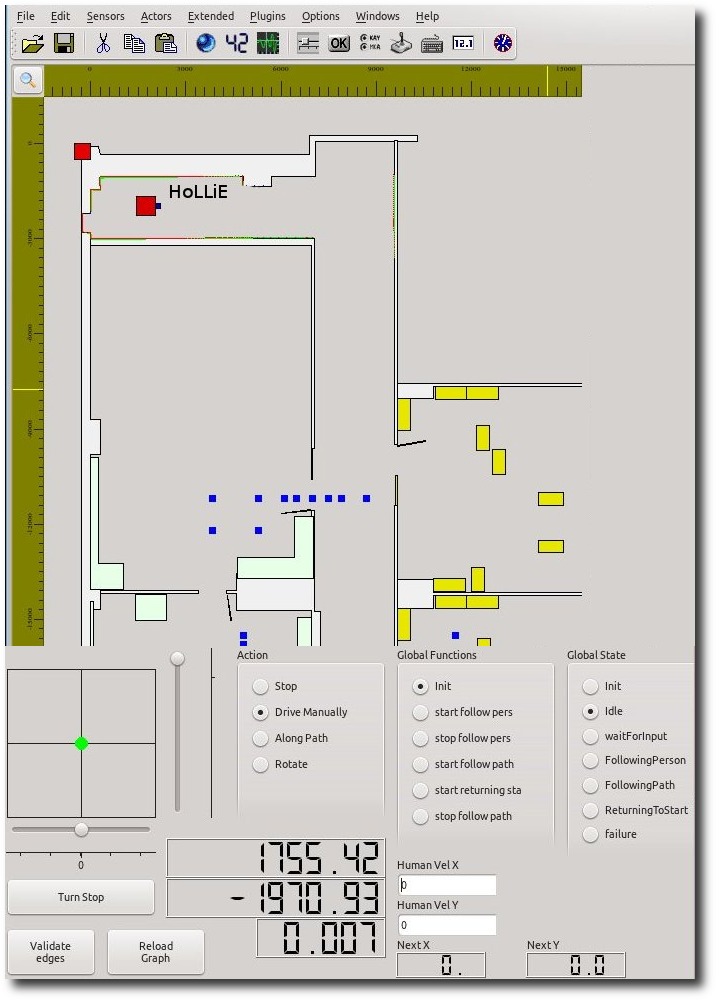
\includegraphics[scale=0.4]{graphics/mcagui_screenshot.png}		
\caption{\label{fig:mcagui} Die entwickelte Simulationsoberfläche
}
\end{figure}

Ein Problem am Anfang war, wie man den zu verfolgenden Mensch simulieren sollte. Um dies zu lösen, benutzt man einfach Mausklicks auf der Karte.
